\documentclass[a4paper,12pt]{report}

\title{Computing Two Point Correlators For A Lattice QCD Theory On Graphics Processor Units}

\author{P\'adraig \'O Conbhu\'\i\\08531749}

%packages
\usepackage[T1]{fontenc}
\usepackage{setspace}
\usepackage{fullpage}

\usepackage{graphicx}
\usepackage{float}
\usepackage{titlepic}

\titlepic{
\includegraphics[width=0.2\textwidth]{images/espiral}}

\usepackage{ marvosym }
\usepackage{verbatim}
\usepackage{amsmath}

\usepackage{array}

\usepackage[savemem]{listings}
\usepackage{color}
 
\definecolor{dkgreen}{rgb}{0,0.6,0}
\definecolor{gray}{rgb}{0.5,0.5,0.5}
\definecolor{mauve}{rgb}{0.58,0,0.82}
 
\lstset{ %
  language=C++,                % the language of the code
  basicstyle=\footnotesize,           % the size of the fonts that are used for the code
  numbers=left,                   % where to put the line-numbers
  numberstyle=\tiny\color{gray},  % the style that is used for the line-numbers
  stepnumber=1,                   % the step between two line-numbers. If it's 1, each line 
                                  % will be numbered
  numbersep=5pt,                  % how far the line-numbers are from the code
  backgroundcolor=\color{white},      % choose the background color. You must add \usepackage{color}
  showspaces=false,               % show spaces adding particular underscores
  showstringspaces=false,         % underline spaces within strings
  showtabs=false,                 % show tabs within strings adding particular underscores
  frame=single,                   % adds a frame around the code
  rulecolor=\color{black},        % if not set, the frame-color may be changed on line-breaks within not-black text (e.g. commens (green here))
  tabsize=4,                      % sets default tabsize to 2 spaces
  captionpos=b,                   % sets the caption-position to bottom
  breaklines=true,                % sets automatic line breaking
  breakatwhitespace=false,        % sets if automatic breaks should only happen at whitespace
  title=\lstname,                   % show the filename of files included with \lstinputlisting;
                                  % also try caption instead of title
  keywordstyle=\color{blue},          % keyword style
  commentstyle=\color{dkgreen},       % comment style
  stringstyle=\color{mauve},         % string literal style
  escapeinside={\%*}{*)},            % if you want to add a comment within your code
  morekeywords={threadIdx,blockIdx,TILE_WIDTH}               % if you want to add more keywords to the set
}


%commands
\def\CPP{{C\kern-.05em\raise.23ex\hbox{+\kern-.05em+}}}
\newcommand{\tr}[1]{\textrm{Tr}\left[ #1 \right]}
\def\flops{{FLOPS}}
\def\gflops{{GFLOPS}}
\newcommand{\ket}[1]{\ensuremath{\left| #1 \right>}} % for Dirac bras
\newcommand{\bra}[1]{\ensuremath{\left< #1 \right|}} % for Dirac kets
\renewcommand{\exp}[1]{\ensuremath{\textrm{e}^{ #1 }}}
\renewcommand{\log}[1]{\ensuremath{\textrm{log}\left( #1 \right)}}

\newenvironment{CUDAtiming}%
{\setlength{\extrarowheight}{1.5pt} \begin{center}\begin{tabular}{l|r} Algorithm & GFLOPS\\\hline}%
{\end{tabular}\end{center}}


\makeatletter
\newcommand\ackname{Acknowledgements}
\if@titlepage
  \newenvironment{acknowledgements}{%
      \titlepage
      \null\vfil
      \@beginparpenalty\@lowpenalty
      \begin{center}%
        \bfseries \ackname
        \@endparpenalty\@M
      \end{center}}%
     {\par\vfil\null\endtitlepage}
\else
  \newenvironment{acknowledgements}{%
      \if@twocolumn
        \section*{\abstractname}%
      \else
        \small
        \begin{center}%
          {\bfseries \ackname\vspace{-.5em}\vspace{\z@}}%
        \end{center}%
        \quotation
      \fi}
      {\if@twocolumn\else\endquotation\fi}
\fi
\makeatother


\begin{document}
\pagenumbering{roman}
\maketitle


\begin{abstract}
An approach to computing two point correlator functions for a Lattice QCD theory is discussed.
Several kernels for use with a CUDA compatible GPU are proposed along with an implementation for these correlation functions.
The multiplication kernels documented here show an increase in \flops{} over the CUBLAS CGEMM routine of up to 35\%.
A tracing kernel is proposed that improves upon a simple dot product approach by potentially two orders of magnitude, as regards \flops{}, by reorganizing several traces with common data into matrix multiplications.
\end{abstract}

\begin{acknowledgements}
I would like to thank Dr. Peardon for continually pointing me in the right direction and for his input and help throughout this project.
The contributions of Tim Harris, Pol Vilaseca Mainar, Graham Moir to my understanding of Lattice QCD through weekly blackboard sessions were enormous and they have my gratitude.
A mention must also be made of the students who sat in on those blackboard sessions.
Further, I would like to thank David Alexander Robinson for his support and encouragement throughout the project.
I suppose I should also mention NVIDIA, without whom there would be no CUDA C on which to base this paper.
\end{acknowledgements}


\tableofcontents



\onehalfspacing

%#########################
%#	Introduction	##
%#########################
\chapter{Introduction}
\pagenumbering{arabic}


%#########################
%#	Motivation	##
%#########################
\section{Motivation}

\subsection{Lattice QCD}
Due to the strength of interaction of the strong force at long distances, perturbative models are not appropriate.
Lattice QCD is an approach to solving problems of quarks and gluons non-perturbatively\cite{Lattice_Methods}.
A lattice of space-time is defined, where quarks are placed on lattice sites and gluons on the connections between them.
A discretized action is used to describe the field theory on the lattice, such that when the lattice spacing $a \rightarrow 0$, it produces a continuum action.

As a non-perturbative theory, lattice QCD is capable of producing exact results from first principles, dealing directly with the path integral formalism.
In practice, however, the accuracy of the theory is limited by computational power.
As the lattice spacing decreases, the computational power required to perform a calculation increases.
Rather than using brute force approaches, more subtle approaches are normally used.



\subsubsection{The Two Point Correlator Function}

The correlator function as defined\cite[p~215]{ Lattice_Methods}
%
\begin{equation}
C_{ij} = \left< O_i O_j \right>
\end{equation}
%
can be used to find the mass of particles.
We're particularly interested in meson correlator functions.
This function can be written in the form of the trace of four matrices multiplied together, so the problem can be passed to a computer to be calculated.

\begin{equation}
C_{ij}(\delta) = \sum_t \tr{\Phi_i(t+\delta)\ \tau(t+\delta, t)\ \Phi^\dagger_j(t)\ \tau(t, t+\delta)}
\end{equation}

We'll be looking here to find an efficient (and more importantly, fast) way of doing this on a GPU.
Some things need to be taken into account to determine whether or not this is worth it.
As it turns out, given the number of flops to perform and the amount of information actually passed to the card, it certainly is worth it.











%#################################
%#	The Parallel Paradigm	##
%#################################
\subsection{The Parallel Paradigm}

As a rule, computers tend to follow Moore's law, named after Intel's Gordon E. Moore, who said\cite{Moores_Law}:
%
\begin{quotation}
The complexity for minimum component costs has increased at a rate of roughly a factor of two per year...
Certainly over the short term this rate can be expected to continue, if not to increase.
Over the longer term, the rate of increase is a bit more uncertain, although there is no reason to believe it will not remain nearly constant for at least 10 years.
That means by 1975, the number of components per integrated circuit for minimum cost will be 65,000.
I believe that such a large circuit can be built on a single wafer.
\end{quotation}
%
However, we are quickly reaching the limits of this prediction\cite{Moore_Limits}.
A reasonable goal is now to find other ways of speeding programs up than simply building faster processors.
This is where the parallel paradigm comes in.

One of the approaches to computing problems involving large numbers of operations is parallel programming.
A parallel program is one that is split into multiple parts and each part run simultaneously, working together to produce some end result.
As such, to solve a problem in a parallel fashion, it is necessary to express it in a manner that can be parallelized.

As one might imagine, if a program can be split perfectly into two parts and run on two processors simultaneously, it should finish in half the time.
In general though, one can't fully parallelize a program, so some of it must execute in a serial manner.
If a fraction $P$ of a code can be fully parallelized and run on $N$ processors, by Amdahl's Law\cite{Amdahls_Law}, the maximum speedup of the program, $S$, over the serial code is given by
%
\begin{equation}
S = \frac{1}{(1-P) + \frac{P}{N} }
\end{equation}

In parallel processors, each processor works independently of the others.
Specifics of memory access and caching is different from processor to processor.
Often it is necessary to write an algorithm quite differently for one family of parallel processors than for another.

There are certain problems much more suited to parallel programming than others.
A parallel program should be capable of being split into multiple sections that each run independent of each other.
However, there is often some overlap necessary in the computations.
Some sections may require the results of some others.
In this case, one goal is to reduce the frequency of these occurrences through some clever trickery and structuring of the program, or to move these synchronizing events to a section where the particular processor the program is being run on allows for it.






\section{General Purpose GPU}

With gaming these days, and general demand in the market for more and more powerful GPU cards, they're becoming more powerful and cheaper as time goes on\cite[p~21]{KirkAndHwu}.
Before any kind of low level API was offered, some people tried to trick GPUs into doing what they wanted.
The use of a GPU for applications other than graphics processing is known as GPGPU\cite[p~7]{KirkAndHwu}.
GPU manufacturers used to just give APIs for doing pixel shadings or rotations, or other graphics related operations.
Some of these can be used to manipulate other matrices in other ways.

Recently, however, NVIDIA has opened up the GPU API to developers to do with the card as they wish.
This is being taken up for scientific applications by many groups.
We wish to do the same.
Using this, it is possible to easily get somewhere around an order of magnitude or two speed increase from a program on a desktop computer\cite[p~10]{KirkAndHwu}.
With this, it may be possible to do calculations that would previously have had to be done on a cluster.

Normally, a cluster is shared by several groups.
Often there are queues to use the clusters.
Often, there are time limits on overall computation time imposed on groups.
By moving some of these jobs to the group's personal computers, they can avoid this queue and avoid using their computation time.
Before, it would have been unfeasible to run some of these programs on desktop computers.
Further, clusters can be quite expensive.
Rather than purchasing a cluster, or paying for time on other clusters, a single NVIDIA Tesla C1060 GPU (on which the tests in this paper were conducted) can, at the time of writing, be bought for about \EUR{1000} (or on eBay for about \EUR{400}!) whereas the TCHPC cost around \EUR{500,000}\cite{TCHPC_cost}.
The difference in pricing here speaks for itself.
In fact, a cluster of Tesla cards can be purchased for somewhere on the order of \EUR{60,000}, which is a much more accessible figure for small groups.




%#########################################
%#	NVIDIA GPU Architechture	##
%#########################################
\chapter{NVIDIA GPU Architecture}

\section{Thread Hierarchy}
A thread is a set of instructions to be run in some order\cite[p~7]{ CUDA_C_Programming_Guide}.
In our case, a thread is a single instance of a kernel running with some particular set of ids associated with it.
Threads are organized into blocks and then from blocks into grids.
When a kernel is run, it generates a grid of blocks, each with a particular block id.
Blocks are placed onto streaming multiprocessors on the card as evenly as possible for execution until there are no blocks left.

Each block has a local block of memory called shared memory that can be accessed by all threads within that block, but only by threads within that block.
This memory has much lower access latency than global memory, and as there are potentially much fewer threads trying to access it, it has potentially much higher bandwidth per thread.

Threads within blocks run somewhat independently of each other.
Threads are organized into warps, each of size 32 threads.
Each thread in the same warp issues an instruction into the pipeline at the same time, however, they do not require the instructions to execute at the same time.
This is important for memory access considerations.
In cases where coalescing or bank conflicts are taken into consideration, one generally considers simultaneous access by threads in the same warp, because memory tends to serve threads of the same warp simultaneously.

Where a kernel requires some synchronization barrier, it is usually best to organize the algorithm such that only threads within the same block need to be synchronized.
This is because blocks cannot speak with each other, save for using some piece of global memory as a flag, say.
It is usually best to avoid global memory accesses as much as possible.

\subsection{Identification}
When executing a kernel on the Host, execution parameters are defined, including the dimensions of the grid and the blocks\cite[p~9]{ CUDA_C_Programming_Guide}.
This is done by passing a value of type dim3, a type provided by CUDA, with the extent of each dimension (up to 3 dimensions for blocks, but only 2 for grids.
Any dimension not specified defaults to 1).
So, say a kernel is launched as
%
\begin{verbatim}
kernel<<<dim3(a,b), dim3(c,d,e)>>>(float *M)
\end{verbatim}
%
when inside the kernel, if one queries \verb!blockIdx.x!, it will return a value between 0 and a-1.
Similarly, \verb!blockIdx.y! returns a value between 0 and b-1.
When querying \verb!threadIdx.x! it will return between 0 and c-1.
Similarly for \verb!.y! and \verb!.z!. Each thread has a unique combination of \verb!blockIdx! and \verb!threadIdx!, and each value is visited.

When a kernel is launched, initially, it attempts to place blocks of increasing \verb!blockIdx.x! onto the SM, followed by \verb!blockIdx.y!, but as the calculation progresses, it is not guaranteed that blocks are executing in order.
In general, it is best not to rely on anything to run in order.

When a block is running, it will group threads into warps.
Threads are assigned to warps first in increasing \verb!threadIdx.x!, then \verb!threadIdx.y! and finally \verb!threadIdx.z!.
Using this knowledge, it is possible to determine which threads will issue instructions simultaneously, so it should be possible to organize an algorithm to avoid any nasty warp level effects like warp serialization or branch divergence.


\section{Memory Hierarchy}
There are several other types of memory that will not be covered in this paper, but we will at least cover what was actually used.

There are 2 main levels of memory to consider: Host memory and Device memory\cite[p~10]{ CUDA_C_Programming_Guide}.
Device memory is then split into 3 levels: Global memory, shared memory and register memory.
These are listed in order of decreasing latency and increasing bandwidth per thread, or more generally, in order of closeness to an executing thread\cite[p~84]{ CUDA_C_Programming_Guide}.
It is usually a good idea to store frequently used memory as close to the thread as possible.
However, as storage gets closer to the thread, more and more restrictions and performance considerations come into play.

\subsection{Global and Local Memory}

Global memory tends to have a large storage space as it is stored off-chip, typically on the order of MBs or GBs.
However, latency of access is around 400 to 800 clock cycles\cite[p~85]{ CUDA_C_Programming_Guide}, and bandwidth is typically around 100~GB/s\cite[p~78]{ KirkAndHwu} on high end cards.

Local memory is stored in the same place, so it has the same qualities\cite[p~89]{ CUDA_C_Programming_Guide}.
Local memory is used if the compiler considers a thread to be using too many registers.
An SM has a limited number of registers that it must share among threads\cite[p~80]{ CUDA_C_Programming_Guide}.
If each thread requests too many registers, the number of threads an SM can service is lowered, so it may be more advantageous to move some of these registers to local memory and hope occupancy is high enough to hide access latency to this memory, and also hope that local memory bandwidth isn't the bottleneck of a kernel, or that is has, at least, been reduced to a reasonable level.

\subsection{Shared Memory}
Shared memory has much reduced capacity, a maximum of 16~KB\cite[p~148]{ CUDA_C_Programming_Guide}, but considering each block potentially requires this much memory independent of other blocks, it's hardly surprising it's somewhat small since a streaming multiprocessor must allocate this much memory to every block currently executing on it.
Latency to this memory depends on your specific hardware, but it is orders of magnitude lower than global memory.
The bandwidth is 32 bits per 2 clock cycles per bank\cite[p~152]{ CUDA_C_Programming_Guide}.

To increase parallel access to shared memory, it is partitioned into 16 banks for cards of compute capability 1.x or 32 banks for compute capability 2.x, each of which can issue data to different threads in a warp simultaneously.
In the case that all threads in a half-warp (for compute capability 1.x) or a whole warp access the same memory address, the bank can broadcast that data to all threads in the warp simultaneously.
Data is organized in the banks such that successive 32 bit words (ie, an int or a float is of size 32 bits) are in successive memory banks.
Therefore, in a half warp for compute capability 1.x or a whole warp for compute capability 2.x, if an array of floats is indexed by threadIdx.x with an odd stride (eg 1), each thread will access a different bank\cite[p~31]{ CUDA_C_Best_Practices_Guide}.
If, however, there is an even stride, some threads will attempt to access different words in the same bank simultaneously.
In this case, warp serialization occurs, where the bank serializes the request, and services the request of each querying thread one by one.
Each bank does this independently of the others, but this can slow a kernel down considerably.


\section{Hardware}
A CUDA card is comprised of a salable number of streaming multiprocessors (SM)\cite[p~79]{ CUDA_C_Programming_Guide}.
Blocks are placed on SMs to be executed.
The SM then organizes the threads of a block into warps to be scheduled for execution.
Each streaming multiprocessor has a number of 32 bit registers and a parallel data cache.
The registers are divided up among the active warps and are the registers used by each thread of the warp.
The parallel data cache is divided up among the blocks running on the SM as their shared memory.
As the registers of a warp remain on the chip, there is no performance penalty for swapping one warp, which may be waiting on some data or some some other operation for example, for another to be executed.
The hardware does this regularly enough, and so it is impossible to determine in exactly what order the threads of a kernel will execute.
The SM is the primary reason for threads to be organized into warps and blocks.

As a block finishes execution, another block is placed onto the SM in its place.
For cards of compute capability 1.x, only one kernel can be executed at a time, so the amount of work that can be done in parallel on a card is limited to the amount of blocks a kernel launches. For compute capability 2.x, kernels can be simultaneously executed.
For these reasons, it is good to have kernels which launch many blocks, whose dimension is a multiple of the warp size, not use too much shared memory, and use as few registers as possible.
It is often, also, a good idea to fuse multiple kernels into one large one, enumerating which kernel run you're currently dealing with using one dimension in \verb!blockIdx!.
This way, there will be many active warps on the card, so as one is waiting for data, the latency of that access can be completely hidden by the execution of another warp.

The maximum number of blocks that can be placed on an SM at any one time, and hence the maximum number of resident warps on an SM, is determined by which condition is first met (all specific to each card): the maximum number of threads allowed per SM, the maximum number of blocks allowed per SM, the maximum amount of shared memory per SM.
Similarly, the maximum number of resident warps will be affected by this and the number of registers used by each thread, as there are a finite amount on the SM.
Specific numbers are not really important, only that they exist, and this sort of thing should be considered in optimizations.

The card runs in an architecture known as SIMT.
This is similar to SIMD vector processors, except it is not necessary for an algorithm to be vectorized.
Threads in a warp are run simultaneously on the SM and instructions are pipelined.
This is one of the reasons why warps can be swapped around for execution on the SM.

It is worth noting that unlike a CPU, there is no branch prediction or speculative execution, so it is worth vectorizing an algorithm, at least to warp granularity.


%#########################################
%#	The CUDA Programming Language	##
%#########################################
\section{The CUDA Programming Language}
The CUDA programming language is the low level API that NVIDIA has provided to developers to write programs to be run explicitly on their GPUs\cite[p~21]{ KirkAndHwu}\cite[p~18]{ CUDA_C_Programming_Guide}.
It is designed to be a simple extension to C (it actually compiles as \CPP{}, however only C style programming and very simple \CPP{} may be used to write kernels run on the GPU), so programmers will be familiar with most of the programming model.
After a short introduction, it should be possible for a programmer to immediately write a kernel to be run on a CUDA enabled GPU.

The main pieces added to C are functionalities to define code that is to run on the Host (the CPU controlling the GPU) and the Device (the GPU on which the kernel is executed).
In device code, there are further specifications as to where particular pointers are mapped: global, local, shared and register memory.
It then provides functions for defining different types of memory, for allocating memory to them, for transferring memory, and also for device synchronizations, as appropriate.

To run a piece of code on a CUDA enabled GPU, a function called a kernel is written.
within this kernel, the programmer is free to define shared memory to be shared between threads in a particular block, local registers for each thread, and then whatever function the programmer wants to write.
Inside the kernel, however, the programmer is limited to functions declared to be capable of running on the device.
In general, if a function is not declared explicitly to run on the device, then it won't.
This means certain handy classes, such as the vector class etc, or any classes the programmer might have written without being careful of avoiding these classes won't work on the card.
One of the main reasons for this is that it is not easy to dynamically allocate memory within a kernel.
And if memory is allocated and the programmer is not careful, it can have some serious performance impacts.


%#########################################
%#	Performance Considerations	##
%#########################################
\section{Performance Considerations}
When writing a kernel, there are multiple potential pitfalls to consider.
They will be listed here with some solutions suggested.
Some can be completely avoided, others only minimized.




\subsection{Bandwidth}\label{subsec:bandwidth}
Each stage of memory transfer has a certain bandwidth associated with it.
This is generally one of the biggest bottlenecks in a kernel and is definitely worth tackling first.

\begin{description}
\item[Coalescing] When a request is coalesced, only one set of data needs to be sent\cite[p~20]{ CUDA_C_Best_Practices_Guide}.
The minimum amount of data that can be queried and sent to a warp is 32 bytes.
So, if a data request asks for less than 32 bytes, or goes outside of a 32 byte word boundary unnecessarily, extra elements will be sent to that warp, while only some of them will be kept and used.
It is therefore more desirable to request only those elements that will be used, requiring data requests to be coalesced.
When data is to be queried from global memory, the programmer should try to have each thread in a warp access a useful element, and have all elements queried in the same word.

\item[Storage Hierarchy] Bandwidth to a thread increases as the storage area gets closer to the chip.
Bandwidth between the host and global memory is lower than between global memory and a thread.
Similarly, global memory to thread bandwidth is lower than shared memory to thread bandwidth.
Finally, the highest bandwidth is for thread registers.
By storing as much memory as close to the chip as possible, effective bandwidth can be reduced.
One must be careful, however, as each area of storage has different restrictions, and they usually become more restrictive as one gets closer to the chip.

\item[Overall Requests] In the case of matrix multiplication, each element in each matrix to be multiplied is called $n$ times, where $n$ is the width of the matrix.
Repeat calling from global memory can be reduced dramatically, compared to a na\"{\i}ve algorithm, by using a tiling algorithm.
This involves each thread block copying an $m\times{m}$ tile from global memory to shared memory, to be used by all the threads in a block.
It can be shown that an $m\times{m}$ tile reduces global memory requests by a factor $m$\cite[p~24]{ KirkAndHwu}\cite[p~18]{ CUDA_C_Programming_Guide}.

\end{description}



\subsection{Latency}\label{subsec:latency}
Any piece of memory queried has a certain latency associated with it.
That is, a certain amount of clock cycles before a memory bank is even ready to start sending some memory.
There are several methods of dealing with latency.
They are listed here in some kind of order.

\begin{description}
\item[Coalescing] By requesting data that resides in the same 32 or 128 byte words, only one request must be made per word.
So, by ordering data requests so they reside entirely in blocks of these words, much fewer requests are made, and so much lower overall latency is involved in these requests.

\item[Occupancy] By having a large number of resident warps to be run, while one warp is waiting for a piece of memory due to latency, another warp can run\cite[p~39]{ CUDA_C_Best_Practices_Guide}.
If that warp has already issued a request and had previously been waiting for some memory due to latency, it can now run.
By having enough resident warps, latency can be well hidden.

\item[Storage Hierarchy] In all cases, it is best to keep as much memory as close to the chip as possible, while simultaneously avoiding nasty effects such as register spilling.
The closer storage is to a thread, the lower its latency.
In the case where a certain piece of memory is used quite often, it might be a good idea to store it in a register or in shared memory.

\item[Prefetching] By requesting the memory needed for the next loop iteration in a looping statement while the current iteration is proceeding, an entire iteration's worth of calculations can be run before the requested memory is needed\cite[p~113]{ KirkAndHwu}.
This can be done because of the SIMT architecture of the CUDA core, meaning the same instruction is issued at the same time for each thread in a warp, but each instruction need not execute at the same time, and each individual thread is independent in this sense.
Since this calculation takes time, the latency for the memory access can be hidden in these operations.
This works because the card doesn't actually wait for the memory to arrive until it is required for some calculation.
In this case, the memory isn't needed until the next iteration of the loop.

\end{description}




\subsection{Overhead}
In some cases, thread overhead can be somewhat large.
There are some things each thread must compute before it can begin.
In some cases a calculation can be organized such that several threads can be combined into one thread in such a way that only one awkward calculation needs to be done at the start of the thread and the numbers that would have been calculated for the other threads are at a simple offset from the first thread.

Care must be taken that this is not overused, because what was once a parallel program can quickly become a serial one.
The optimum number for this is often quite small.

Kernel launch overhead can also be large\cite[p~187]{ KirkAndHwu}, so in the case where a kernel is run multiple times, if the kernel launches can be parallelized, it can be a good idea to merge several launches into the one kernel.
By passing the appropriate data and enumerating kernels using one of the \verb!blockIdx!, this can be a very simple improvement to implement.


\subsection{Calculation Reduction}
It is often desirable to reduce the actual number of operations performed by a thread.
There are a few ways of approaching this.

\begin{description}
\item[Loop Unrolling] The nvcc compiler provides a \verb!#pragma unroll! option\cite[p~95]{ CUDA_C_Programming_Guide}.
This will write out a loop explicitly, inserting a number where the iterator would have been for each iteration.
This reduces both the number of registers required by a thread and also the number of calculations needed to be done by the thread.
In the case of some conditional statement depending on the iterator, these can be computed explicitly by the compiler, further reducing the number of calculations performed.
If the loop to be unrolled would be too long, causing too much code expansion, the compiler returns a warning to that effect.

\item[Load Spreading] In the case where some numbers computed by several threads need to be added together, one solution is to write these to shared memory and have thread 0 do all the adding.
Another option, to reduce the load on thread 0, is to do some sort of shared summation.
It can be set up that each thread writes their value to shared memory, and then for some loop running an appropriate length, the first half of the thread block add their value and the next half's value and writes it back to shared memory, then the first quarter read theirs and the second quarter's values etc until there is only 1 thread left.
Using threads in this manner falls within the general idea of parallel programming, so it should come as no surprise that it is preferred to perform these sorts of calculations in a parallel manner if possible.
However, the lazy "make thread 0 do everything" approach is handy for debugging.
\end{description}


\subsection{Serialization}
One must be careful to access memory banks in a parallelizable manner\cite[p~26]{ CUDA_C_Best_Practices_Guide}.
Both global and shared memory is divided into banks of memory.
When a warp is accessing a memory bank, the accesses must be organized such that each thread in the warp accesses either the same word in a bank as another thread, or a different bank altogether.
In the case two threads access two different words in the same bank, the request must be serialized into two conflict free requests.
So instead of one transaction occurring, two transactions must occur, and the second one must wait for the first to complete before proceeding.
This reduces access speed and should be avoided.

One must also be aware of branch divergence\cite[p~95]{ CUDA_C_Programming_Guide}.
In the case where there is some control flow in a kernel, one should try to have every thread in the same warp follow the same path.
For each different path followed by threads in a warp, the warp must be passed through the SM for execution during the divergence.
So, in the case where threads in a warp diverge down two paths for some duration, this section must be executed twice, once for each path, thus increasing the overall execution time of the warp.


\subsection{Instructions}
For some operations, there exist several different possibilities for their execution\cite[p~46]{ CUDA_C_Best_Practices_Guide}.
By selecting the appropriate operation, it may be possible to speed a program up (or slow it down!).
For example, on the card, there exists a fused multiply-add operation (FMAD) which computes a multiplication and addition in one operation, rather than the usual two.
However, for devices of compute capability 1.x, it is not IEEE-754 compliant.
After performing the multiplication, the result is simply truncated rather than rounded when put into the sum.
Therefore, it is possible a kernel might return a result that differs from some serial CPU code.
There are multiplication and addition operators that can be used to specify explicit multiplications and explicit additions, to avoid the compiler optimizing a multiply-add into a FMAD.

There exist circumstances where speed is more important than accuracy, and CUDA cards provide for this.
There are some operations such as \verb!sin()! and \verb!cos()! that have alternate versions \verb!__sin()! and \verb!__cos()! which map directly to the hardware, and hence take much fewer clock cycles to compute, but they're less accurate.
Worse, they're only somewhat accurate within a certain range of the argument.



\chapter{Formulating The Correlation Functions}
\label{chap:correlation_functions}

\section{Energy Eigenvalues}
Given the correlator\cite[p~215]{Lattice_Methods}
%
\begin{equation}
C_{ij}(\delta) = \bra{0} \Phi_i(\delta) \Phi^\dagger_j(0) \ket{0}
\end{equation}
%
Switching to the Heisenberg picture yields
%
\begin{align}
C_{ij}(\delta) 	&= \bra{0} \exp{\hat{H}\delta} \Phi_i \exp{-\hat{H}\delta} \exp{\hat{H}0} \Phi^\dagger_j \exp{-\hat{H}0} \ket{0}\\
%
		&= \bra{0} \Phi_i \exp{-\hat{H} \delta} \Phi^\dagger_j \ket{0}
\end{align}
%
Inserting a complete set of states, we get
%
\begin{align}
C_{ij}(\delta) 	&= \sum_n\ \bra{0} \Phi_i(0) \exp{-\hat{H} \delta} \ket{n}\bra{n} \Phi^\dagger_j(0) \ket{0}\\
%
		&= \sum_n\ \bra{0} \Phi_i(0) \ket{n} \exp{-E_n \delta} \bra{n} \Phi^\dagger_j(0) \ket{0}
\end{align}
%
We now label
%
\begin{align}
\bra{0} \Phi_i(0) \ket{n} &= Z_{in}\\
\bra{n} \Phi^\dagger_j(0) \ket{0} &= Z^\dagger_{nj}\\
\delta^n_k \exp{-E_n \delta} &= D_{nk}(\delta)
\end{align}
%
$D_{nk}$ is a matrix whose diagonal elements are the energy eigenvalues of the inserted states, and all other elements are 0.

We may now rewrite the correlator in the matrix form
%
\begin{align}
C_{ij}(\delta) 		&= Z_{in} D_{nk}(\delta) Z^\dagger_{kj}\\
C(\delta) 	&= Z D(\delta) Z^\dagger\\
			&= Z (Z^\dagger (Z^\dagger)^{-1}) D(\delta) Z^\dagger
\end{align}
%
Since $Z Z^\dagger = C(0)$, we have
%
\begin{equation}
C(\delta) = C(0) (Z^\dagger)^{-1} D(\delta) Z^\dagger
\end{equation}
%
Now, $(Z^\dagger)^{-1} D(\delta) Z^\dagger$ has the same eigenvalues as $D(\delta)$, which are $\lambda_n(\delta) = \exp{-E_n \delta}$, so we get the generalized eigenvalue equation
%
\begin{align}
C(\delta)\vec{v}_n 	&= C(0) ((Z^\dagger)^{-1} D(\delta) Z^\dagger) \vec{v}_n\\
			&= C(0) \lambda_n(\delta) \vec{v}_n\\
			&= C(0) \exp{-E_n \delta} \vec{v}_n
\end{align}
%
Thus, the energy can be found:
%
\begin{equation}
E_n = \log{\lambda(\delta)/\lambda(\delta+1)}
\end{equation}

This simultaneously eliminates the difficulty in finding excitation values using correlators and improves the signal to noise ratio.
As one can see from here, if only one observable is used, only 1 energy level, the ground energy, can be correctly determined.
Further, it has only been determined using one source of data.
Generating is using more sources of data should, therefore, improve the accuracy of each level found.

It remains to actually compute a correlator matrix.




\section{Matrix Representation of the Correlator}
We consider the correlation function\cite[p~217]{ Lattice_Methods}
%
\begin{equation}
C(t) = \sum_x \left< O(t) O(0) \right>
\end{equation}
%
where $O(t)$ is an observable that looks like a meson with some particular quantum numbers.
Specifically, some fermionic fields, $\psi^\alpha_i(t)$ where the roman index denotes spin and the Greek index denotes colour sandwiching some Dirac matrices, $\Gamma_{ij}$
%
\begin{equation}
O(t) = \bar{\psi}(t) \Gamma \psi(t)
\end{equation}
%
Expanding, the correlator gives
%
\begin{equation}
C(t) = \bra{0} \bar{\psi}^\alpha_i(t) \Gamma_{ij} \psi^\alpha_j(t) \bar{\psi}^\beta_k(0) \Gamma_{kl} \psi^\beta_l(0) \ket{0}
\end{equation}
%
We define
%
\begin{equation}
\bra{0} \psi^\alpha_j(t_1) \bar{\psi}^\beta_k(t_2) \ket{0} = G^{\alpha \beta}_{j k}(t_1,t_t)
\end{equation}
%
as it turns out\cite[p~52]{Lattice_Methods},
%
\begin{equation}
G(t_1,t_2) = M^{-1}_{F_{t_1 t_2}}
\end{equation}
%
where $M_{F_{t_1 t_2}}$ is the fermion propagator.

Normal ordering, and remembering sign changes due to the use of Grassman variables produces the result
%
\begin{equation}
C(t) = \tr{G(t,t) \Gamma} \tr{G(0,0)\Gamma} - \tr{G(t,0)\Gamma G(0,t) \Gamma}
\end{equation}

In the case of a flavour nonsinglet, the first term evaluates to zero\cite[p~218]{Lattice_Methods}, so finally we have (dropping the minus sign)
%
\begin{align}\label{eqn:wrong_correlator}
C(t) 	&= \tr{G(t,0)\Gamma G(0,t) \Gamma}\\
	&= \tr{\Gamma G(t,0) \Gamma G(0,t)}
\end{align}

We use a slightly modified version of this correlator
%
\begin{equation}\label{eqn:right_correlator}
C_{ij}(\delta) = \sum_t \tr{\Phi_i(t+\delta) G(t+\delta,t) \Phi^\dagger_j(t) G(t, t+\delta)}
\end{equation}
%
whose derivation follows similar steps.
We perform the sum over $t$ because we are on a lattice with periodic boundary conditions, so our choice of zero time is arbitrary.
By doing this summation, we effectively find an average value for the correlator over all possible starting positions, improving our signal to noise without having to compute extra $\Phi$ matrices.

A database of $\Phi$ matrices and propagators have been computed prior to writing this paper.





%#########################################
%#	A GPU Based Implementation	##
%#########################################
\chapter{A GPU Based Implementation}

Equation \ref{eqn:right_correlator} leaves us with a linear algebra problem that we can tackle computationally.
The general outline we will take is as follows:
%
\begin{align}\label{eqn:correlator_multiply}
	\Phi_i(t+\delta)\ \tau(t+\delta, t) &= X^L_i(t,\delta)\\
	\Phi^\dagger_j(t)\ \tau(t, t+\delta) &= X^R_j(t,\delta)\\
	C_{ij}(t,\delta) &= \tr{X^L_i(t,\delta)\ X^R_j(t,\delta)} \\
	C_{ij}(\delta) &= \sum_{t=0}^{t_{\textrm{max}}} C_{ij}(t,\delta)
\end{align}

By using the relation for time reversal of propagators
%
\begin{equation}\label{eqn:propagator_reversal}
	\tau(t, t+\delta) = \gamma_5\ \tau^\dagger(t+d, t)\ \gamma_5
\end{equation}
%
we can reduce the number of propagators that need to be loaded for each run.
It is conceivable that if two propagators are loaded that two elements of $C_{ij} (t,d)$ could be calculated, but it is easier to keep track of just one.
In the basis used for this calculation, a $\gamma_5$ multiplication requires just one or two extra lines of code to implement, so it is essentially free.

We are now faced with performing two matrix multiplications and a trace of two matrices to compute one time slice of the correlator matrix.


\section{Operation Time vs Transfer Time}
It must be determined whether or not it is worth performing this calculation on a GPU.
As there is quite a low bandwidth across the PCI bus, we must compare the time it takes to move the elements from the host to the device and the number of calculations performed on the device.
We define the Operation/Transfer ratio (O/T) as the number of operations performed divided by the number of elements transferred.
Assuming the time required for each is roughly linearly dependent on these numbers, it's a reasonable ratio to consider.

Assuming two $\Phi$ matrices and one $\tau$ matrix is uploaded for each calculation, and assuming intermediate matrices are kept and/or summed on the card until the final $C_{ij}(d)$ is calculated (so we will ignore this), we have for each time slice calculation:

\begin{center}
\begin{tabular}{r l}
Transfers: & $3N^2$\\
Operations: & $2N^3 + N^2$
\end{tabular}
\end{center}

\noindent giving us a O/T of $\sim \frac{2}{3}N$.
The O/T can be improved to $\sim \frac{4}{3}N$ by calculating $C_{ji}(t,d)$ along with $C_{ij}(t,d)$.
It can be even further improved by loading multiple $\Phi_i$s on to calculate other $C_{ij}$ elements.
Assuming $C_{ij}$ has a width $c$, we get

\begin{center}
\begin{tabular}{r l}
Transfers: & $(c+1)N^2$\\
Operations: & $(2c)N^3 + (c^2)N^2$
\end{tabular}
\end{center}

\noindent and the O/T is $\sim 2N+c$.
As can be seen, when $c \sim N$, this becomes an $N^4$ operation.
With a general O/T of $\sim N$, this is certainly worth while calculating on the GPU.
Compare this to, say, a matrix addition which has an O/T of $\sim 1$, which does not justify the transfer time.

For large N and large c, the transfer time pales in comparison to the operation time.


\section{The Matrix Multiplication Kernels}

Here, we will go through the iterative process of writing a basic kernel and then considering the current bottlenecks and attempting to fix them.

For matrix multiplications, we will use, as our goal, the Flops count of the equivalent CUBLAS operation, CGEMM.

\begin{CUDAtiming}
CGEMM & 219.45
\end{CUDAtiming}

\subsection{The Na\"{\i}ve Implementation}

\begin{lstlisting}[float,caption=Na\"{\i}ve Matrix Multiplication Kernel, label=lst:naive_kernel]
void NaiveMultiply(const cuFloatComplex *A, const cuFloatComplex *B, cuFloatComplex *C, int width)
{
const uint Row = blockIdx.y*TILE_WIDTH + threadIdx.y;
const uint Col = blockIdx.x*TILE_WIDTH + threadIdx.x;

cuFloatComplex Xtmp = make_cuFloatComplex(0,0);

for(int k=0; k<width; k++)
	{
	Xtmp = cuCaddf(
			cuCmulf(
				A[ Row*width + k ],
				B[ k*width + Col ]
				),
			Xtmp ); 
	}

C[Row*width + Col] = Xtmp;
}
\end{lstlisting}

The na{\"\i}ve multiplication kernel in Listing \ref{lst:naive_kernel} suffers from some serious bottlenecks.
Running a comparison test results in the following table.

\begin{CUDAtiming}
CGEMM & 219.45\\
Na{\"\i}ve & 34.09
\end{CUDAtiming}

As discussed in section \ref{subsec:bandwidth}, one of the most important things to tackle are coalescing and overall throughput.
Considering the C1060 has a total global bandwidth of 102.4 GB/s, assuming we call complex floats of 8 bits for each matrix element, and assuming 2 elements are needed for each floating point operation, we say we transfer 16 bits per 8 FLOPs (since complex multiplication requires 8 operations: 4 multiplications and 4 additions).
So, we have a theoretical maximum of $102.4/16 = 6.4$ complex multiplications per second which is $6.4 \times 8 = 51.2$ \gflops{}.
This is around the 34.09 \gflops{} we see.
Compare this to CGEMM which reaches 200 \gflops{}.
So, it is likely global memory bandwidth is the bottleneck we need to tackle.

We introduce a tiled algorithm to take care of both coalescing and bandwidth.


\subsection{The Basic Tiled Algorithm}

\begin{lstlisting}[float,caption=Simple Tiled Matrix Multiplication Kernel, label=lst:simpleTiled_kernel]
void SimpleTiledMultiply(const cuFloatComplex *A, const cuFloatComplex *B, cuFloatComplex *C, int width)
{
const uint Row = blockIdx.y*TILE_WIDTH + threadIdx.y;
const uint Col = blockIdx.x*TILE_WIDTH + threadIdx.x;

__shared__ cuFloatComplex Ash[TILE_WIDTH][TILE_WIDTH];
__shared__ cuFloatComplex Bsh[TILE_WIDTH][TILE_WIDTH];

cuFloatComplex Xtmp = make_cuFloatComplex(0,0);

#pragma unroll
for(int m=0; m<gridDim.x; m++)
	{
	Ash[threadIdx.y][threadIdx.x] =
		A[Row*width + m*TILE_WIDTH + threadIdx.x];
	
	Bsh[threadIdx.y][threadIdx.x] =
		B[(m*TILE_WIDTH + threadIdx.y)*width + Col];
	
	__syncthreads();

	#pragma unroll
	for(int k=0; k<TILE_WIDTH; k++)
		{
		Xtmp = cuCaddf(
				cuCmulf(
					Ash[threadIdx.y][k],
					Bsh[k][threadIdx.x]
					),
				Xtmp
				); 
		}
	__syncthreads();
	}

C[Row*width + Col] = Xtmp;
}
\end{lstlisting}

As can be seen in Listing \ref{lst:simpleTiled_kernel}, the complexity significantly rises in this implementation, however, the \flops{} show significant improvement.

\begin{CUDAtiming}
CGEMM & 219.45\\
Na{\"\i}ve & 34.09\\
Simple Tiled & 177.71
\end{CUDAtiming}


This algorithm takes care of most of the bottlenecks a matrix multiplication algorithm might encounter fairly well.
The idea behind the algorithm is quite simple, but quite effective.

The resulting matrix is split up into tiles of width \verb!TILE_WIDTH!, matching the dimensions of the block, so now there are
$($\verb!width/TILE_WIDTH!$)^2$ tiles to be calculated.
A block of threads collaborates to compute the elements of a tile, so individual blocks correspond directly to individual tiles.
The tile width is chosen such that the data needed to compute it can be stored in a block's shared memory, at least in an iterative manner.

Tiles are loaded from the left matrix in a manner traversing a row of the matrix while tiles are loaded from the right matrix in a manner traversing a column.
This looks much like a matrix multiplication, where the elements of the matrix to be multiplied are, themselves, matrices; i.e.
the loaded tiles.
As a tile can be stored in the shared memory of a block, the matrix multiplication between these tiles can be carried out much quicker from shared memory than it could have been otherwise.
As stated in section \ref{subsec:bandwidth}, a tile of size $m \times m$ reduces global memory requests by a factor of $m$.

By comparing the theoretical new speed, $34.09 \times 16 = 545.44$ \gflops{} to the actual new speed, $177.71$ \gflops{}, we can see that we got about an order of magnitude speedup, as we would expect, but that there is still room for improvement.

Inspecting the output from the visual profiler that comes with the CUDA SDK, computeprof, we see some interesting results.
One is that our occupancy has gone from 1, in the case of the na{\"\i}ve kernel to 0.75.
Since that profiler seems to count in chunks of 0.25, we can't come to too many conclusions based on this.

Another point is that our register count for the kernel has risen from 12 to 14, which is to be expected with the introduction of two new pointers.
This 14 is, however, the same number that CUBLAS uses for its CGEMM routine, so we'll assume this is an optimal amount.There is some importance to this.
There is a maximum number of threads, blocks and registers that can be present on a particular streaming multiprocessor on the device.
This means, if one has too many registers in a thread, fewer threads will be able to run on the device.
This reduces the number of active warps available for the device.
Hence the drop in occupancy observed.
However, this drop in occupancy is greatly outmatched by the increase in \flops{}.

Another noteworthy thing is the number of coalesced loads and stores.
In the na{\"\i}ve kernel, there were high numbers of 32 byte and 128 byte loads and 128 byte stores.
The appearance of 32 byte loads, in our case, indicates poor loading patterns, as it should be possible to have only 128 byte loads.
Indeed, the tiled algorithm achieves this with not only entirely 128 byte loads, but an order of magnitude fewer loads, as expected.
The number of loads in this kernel is the same as the CGEMM kernel.

Finally, a point to note, a large difference between our kernel and the CGEMM kernel is the warp serialization.
Ours is on the order of $10,000$, meaning $10,000$ requests to shared memory had to be serialized and executed sequentially.
Compare this to the CGEMM kernel, which is 0.
Obviously, this is an entirely avoidable problem, so we should tackle this next.


\subsection{Eliminating Warp Serialization}
\begin{lstlisting}[float,caption=Tiled Matrix Multiplication Kernel Without Warp Serialization, label=lst:noSerialization_kernel]
void TiledNoSerializationMultiply(const cuFloatComplex *A, const cuFloatComplex *B, cuFloatComplex *C, int width)
{
const uint Row = blockIdx.y*TILE_WIDTH + threadIdx.y;
const uint Col = blockIdx.x*TILE_WIDTH + threadIdx.x;

__shared__ float Ash[TILE_WIDTH][2*TILE_WIDTH +1];
__shared__ float Bsh[TILE_WIDTH][2*TILE_WIDTH +1];

cuFloatComplex Xtmp = make_cuFloatComplex(0,0);

#pragma unroll
for(int m=0; m<gridDim.x; m++)
	{
	Ash[threadIdx.y][threadIdx.x] =
		cuCrealf(A[Row*width + m*TILE_WIDTH + threadIdx.x]);
	Ash[threadIdx.y][threadIdx.x +TILE_WIDTH] =
		cuCimagf(A[Row*width + m*TILE_WIDTH + threadIdx.x]);
	
	Bsh[threadIdx.y][threadIdx.x] =
		cuCrealf(B[(m*TILE_WIDTH + threadIdx.y)*width + Col]);
	Bsh[threadIdx.y][threadIdx.x +TILE_WIDTH] =
		cuCimagf(B[(m*TILE_WIDTH + threadIdx.y)*width + Col]);
	
	__syncthreads();

	#pragma unroll
	for(int k=0; k<TILE_WIDTH; k++)
		{
		Xtmp = make_cuFloatComplex(
			cuCrealf(Xtmp) +
			Ash[threadIdx.y][k]*Bsh[k][threadIdx.x] -
			Ash[threadIdx.y][k +TILE_WIDTH]*Bsh[k][threadIdx.x +TILE_WIDTH],
			
			cuCimagf(Xtmp) +
			Ash[threadIdx.y][k +TILE_WIDTH]*Bsh[k][threadIdx.x] +
			Ash[threadIdx.y][k]*Bsh[k][threadIdx.x +TILE_WIDTH]
			);
		}
	__syncthreads();
	}

C[Row*width + Col] = Xtmp;
}
\end{lstlisting}

We must look at what happens when attempting to access the tile in shared memory on a card of compute capability 1.x. If a $16 \times 16$ tile is stored in shared memory as \verb!Ash[TILE_WIDTH][TILE_WIDTH]!, when traversing the right bracket, the array goes across memory banks.
However, when traversing the left bracket, the array goes down the same memory bank, since it jumps a length \verb!TILE_WIDTH! each time, which is of size 16.
The trick is to pad the right index by 1 to \verb!Ash[TILE_WIDTH][TILE_WIDTH+1]!.
So, now, when traversing the right bracket, one moves across memory banks, and then traversing the left bracket, one returns to the same memory bank plus 1, so one also moves across memory banks.
Since the extra 1 can effectively be ignored, the array appears and behaves exactly as before, except the transpose of the array can also be accessed easily without warp serialization.

Further consideration must be made for complex numbers.
In general, a stride in shared memory across 32 bit words must be odd (ie, if indexing an array of floats by \verb!s*threadIdx.x!, \verb!s! must be odd).
This isn't possible using a structure like cuFloatComplex which stores 2 floats side by side.
What can be done, however, is to store the real and imaginary parts of a number in different arrays, or in different sections of the same array.
Here, we've declared an array \verb!Ash[TILE_WIDTH][2*TILE_WIDTH+1]!, so the real part can be kept in the first half of the row and the complex part in the second half.
The \verb!+1! here is to facilitate transpose indexing.
By making the change above, we find the following:

\begin{CUDAtiming}
CGEMM & 219.45\\
Na{\"\i}ve & 34.09\\
Simple Tiled & 177.71\\
No Serialization & 217.33
\end{CUDAtiming}

A 22\%
speed increase!As can be seen, this is now near the same speed as CGEMM.
Looking to computeprof once again, there are two differences visible there.
One is that this kernel uses one fewer registers, but since the nvcc compiler is somewhat fickle, we won't make a big deal of this.
However, the number of instructions issued by each kernel is somewhat interesting.
CGEMM issues around 155540 instructions, while ours issues 156410, around 0.5\%
extra while the speed difference is around 1\%
worse.
We should see if there are any unnecessary operations being performed that we should only need to computed once, without using any extra registers, since we're trying to keep them to a minimum.


\subsection{Pointer Iteration}
\begin{lstlisting}[float,caption=Tiled Matrix Multiplication Kernel Using Pointer Iteration, label=lst:pointerIteration_kernel]
void PointerIterateMultiply(const cuFloatComplex *A, const cuFloatComplex *B, cuFloatComplex *C, int width)
{
//const uint Row = blockIdx.y*TILE_WIDTH + threadIdx.y;
//const uint Col = blockIdx.x*TILE_WIDTH + threadIdx.x;

A += (blockIdx.y*TILE_WIDTH + threadIdx.y)*width + threadIdx.x;
B += threadIdx.y*width + (blockIdx.x*TILE_WIDTH + threadIdx.x);
C += (blockIdx.y*TILE_WIDTH + threadIdx.y)*width + (blockIdx.x*TILE_WIDTH + threadIdx.x);

__shared__ float Ash[TILE_WIDTH][2*TILE_WIDTH +1];
__shared__ float Bsh[TILE_WIDTH][2*TILE_WIDTH +1];

cuFloatComplex Xtmp = make_cuFloatComplex(0,0);

#pragma unroll
for(int m=0; m<gridDim.x; m++, A+=TILE_WIDTH, B+=TILE_WIDTH*width)
	{
	Ash[threadIdx.y][threadIdx.x] =
		cuCrealf(A[0]);
	Ash[threadIdx.y][threadIdx.x +TILE_WIDTH] =
		cuCimagf(A[0]);
	
	Bsh[threadIdx.y][threadIdx.x] =
		cuCrealf(B[0]);
	Bsh[threadIdx.y][threadIdx.x +TILE_WIDTH] =
		cuCimagf(B[0]);
	
	__syncthreads();


	#pragma unroll
	for(int k=0; k<TILE_WIDTH; k++)
		{
		Xtmp = make_cuFloatComplex(
			cuCrealf(Xtmp) +
			Ash[threadIdx.y][k]*Bsh[k][threadIdx.x] -
			Ash[threadIdx.y][k +TILE_WIDTH]*Bsh[k][threadIdx.x +TILE_WIDTH],
			
			cuCimagf(Xtmp) +
			Ash[threadIdx.y][k +TILE_WIDTH]*Bsh[k][threadIdx.x] +
			Ash[threadIdx.y][k]*Bsh[k][threadIdx.x +TILE_WIDTH]
			);
		}
	__syncthreads();
	}

C[0] = Xtmp;
}
\end{lstlisting}

Such a seemingly trivial change puts us just past our goal.

\begin{CUDAtiming}
CGEMM & 219.45\\
Na{\"\i}ve & 34.09\\
Simple Tiled & 177.71\\
No Serialization & 217.33\\
Pointer Iteration & 222.67
\end{CUDAtiming}

Instead of having to do a bunch of multiplication and addition operations on each iteration of the \verb!m! loop, we've integrated the numbers that are always added in the same way into the original pointer at the start of the kernel.
Then, instead of having to calculate some shift along the row or vector direction, it's incorporated into the for loop.
The row and col variables have been left for reference in future edits.

As can be seen, this has a 1.5\%
speed improvement over the CGEMM routine, and the computeprof output says it issues around 1-2\%
fewer instructions.

For the sake of curiosity, we'll see what else we can do to improve our time.


\subsection{Prefetching}
Global prefetching requires a little upheaval of the kernel, but it is simple enough to follow.
The basic loop is\cite[p~114]{ KirkAndHwu}:

\begin{enumerate}
\item Load value queried from high latency from previous iteration into lower latency memory.

\item Query value from high latency memory to be used in next iteration.

\item\label{lst:performCalculation} Perform calculation using the values loaded into the lower latency memory.
\end{enumerate}

This is particularly effective if step \ref{lst:performCalculation} is a long calculation.

The 0th element might be loaded into the query variable before the loop begins to avoid any awkward conditional statements needing to be evaluated on each iteration.
If the loop is unfolded, it is possible the awkward conditional statements will be evaluated at compile time, though.
In some cases some pre-loop and post-loop operations will need to be done to ensure the whole loop has been evaluated properly.

The kernel was a bit long to include here.
An attempt was made to write a loop with awkward conditional statements as described above to make it fit, but it seems the nvcc compiler wasn't quite smart enough to evaluate them explicitly when the loop is unrolled, resulting in them being evaluated on each iteration, and slowing the kernel down by about 7\%.
As a result, it has been left an exercise for the reader.
The resulting values for performing a prefetch from global memory and a prefetch from local memory are as follows

\begin{CUDAtiming}
CGEMM & 219.45\\
Na{\"\i}ve & 34.09\\
Simple Tiled & 177.71\\
No Serialization & 217.33\\
Pointer Iteration & 222.67\\
Global Prefetch & 224.17\\
Share Prefetch & 210.71
\end{CUDAtiming}

As can be seen, a global memory prefetch offers a slight speed improvement, while a shared memory prefetch is actually detrimental.
The reason for the share prefetch being detrimental is because of the extra operations needed to perform it, the extra registers needed to hold the queried and more local values, and the fact that there's not many operations between loading each value from shared memory, so the latency can't really be hidden.

The global memory prefetch offers only a marginal improvement because we already have plenty of active warps waiting to perform calculations, so while one warp is waiting for some data from global memory, another warp can be executed.
The prefetch reduces the number of warps needed to hide the latency of the global memory request, thus improving speed a little.


\subsection{Multiplication Fusion}
Considering the task at hand, we have one propagator multiplied with several observables.
It might, therefore, be worthwhile multiplying multiple matrices with the same propagator in the same kernel.
It is a simple extension to the previous kernels.
Instead of just \verb!Ash! shared matrices, we have \verb!A1sh! and \verb!A2sh! shared matrices, pass two matrices, \verb!A1! and \verb!A2!, one propagator matrix, \verb!B!, along with two output matrices \verb!C1! and \verb!C2!.

This was done for two, three and four matrices, with and without prefetching.

\begin{CUDAtiming}
CGEMM & 219.45\\
Na{\"\i}ve & 34.09\\
Simple Tiled & 177.71\\
No Serialization & 217.33\\
Pointer Iteration & 222.67\\
Global Prefetch & 224.17\\
Share Prefetch & 210.71\\
\hline
Double & 240.65\\
Double Prefetch & 256.29\\
Triple & 228.42\\
Triple Prefetch & 257.91\\
Quadruple Prefetch & 240.21\\
Double Double Prefetch & 269.22
\end{CUDAtiming}

A double multiplication should be loading 3 matrices from global memory rather than 4.
This should offer an improvement of around 25\%.
Similarly, a triple multiplication and quadruple should have an improvement of 33\% and 37.5\% respectively.
This isn't quite reflected in the \flops{} though.
While the double multiplication with prefetching offers around 14\%
improvement over the Global Prefetch kernel, which is somewhat near to the 25\%
we'd expect, the triple and quadruple kernels don't improve upon this, and in fact start to decline in performance.
This suggests that global bandwidth isn't necessarily the greatest bottleneck.
With these kernels, register use is increased to around 20, and, according to computeprof, the occupancy is around 50\%.
It is worth noting that an occupancy of around 50\% can be sufficient to hide global access memory latency.
Considering computeprof shows no signs of poor coalescing or warp serialization, the problem is likely latency, bandwidth or overhead related.

Returning to the double kernel, by creating a quadruple kernel by fusing two double kernels, we get all the benefits of a double kernel with some of the overhead of the two double kernels fused into one.
So, as can be seen, with this sort of loop fusion, the double double offers a 5\%
improvement over the single double kernel, a 12\%
improvement over the regular quadruple kernel, and overall, a 20\%
improvement over the Global prefetch kernel, or previously fastest single multiplication kernel.

As can be seen, double and triple etc matrix combining is well worth the effort.
It is surprising how much extra speed prefetching offers.
It is likely prefetching relieves some of the pressure on global memory, allowing the memory to be transferred any time between the first and second matrix multiplications, along with reducing the number of resident warps necessary to hide latency.
There seems to be a peak around two and three multiplications, which is fine, because most problems of this type involving more than one multiplication can be decomposed into groups of two and three multiplications.
The same effect can be seen in the Quadruple and Double Double kernels.
The Quadruple kernel is calling many more elements simultaneously, but only 15\% fewer elements overall, so it's likely this bandwidth clogging is a worse bottleneck than the number of elements passed.

\subsubsection{Another Kind Of Fusion}
\begin{lstlisting}[float,caption=Fused Matrix Multiplication Kernel, label=lst:fused_kernel]
void VectorizedMultiply(const cuFloatComplex *A, const cuFloatComplex *B, cuFloatComplex *C, int width)
{
//const uint Row = ((blockIdx.x/(width/TILE_WIDTH))*TILE_WIDTH + threadIdx.y;
//const uint Col = ((blockIdx.x%(width/TILE_WIDTH))*TILE_WIDTH + threadIdx.x;


A += ((blockIdx.x/(width/TILE_WIDTH))*TILE_WIDTH + threadIdx.y)*width + threadIdx.x  + blockIdx.y*width*width;
B += threadIdx.y*width + ((blockIdx.x%(width/TILE_WIDTH))*TILE_WIDTH + threadIdx.x);
C += ((blockIdx.x/(width/TILE_WIDTH))*TILE_WIDTH + threadIdx.y)*width + ((blockIdx.x%(width/TILE_WIDTH))*TILE_WIDTH + threadIdx.x)  + blockIdx.y*width*width;

//some declarations

#pragma unroll
for(int m=1; m<(width/TILE_WIDTH); m++)
	{
	//the rest of this loop
	}
//the rest of this code
}
\end{lstlisting}
We consider fusing multiple kernels into one kernel, such that instead of calling $2 \times c$ kernels, we write one kernel that multiplies $c$ matrices together.
In our case, we'll only move across the left matrix, since we use the same propagator for all $c$ multiplications.
Only a small change is needed. The execution configuration changes from
\begin{lstlisting}
FusedMultiply<<<dim3(width/TILE_WIDTH,width/TILE_WIDTH), dim3(TILE_WIDTH,TILE_WIDTH)(A,B,C,width)
\end{lstlisting}
to
\begin{lstlisting}
FusedMultiply<<<dim3(width/TILE_WIDTH*width/TILE_WIDTH, cWidth), dim3(TILE_WIDTH,TILE_WIDTH)(A,B,C,width)
\end{lstlisting}
and the change to the kernel is shown in Listing \ref{lst:fused_kernel}.

We write a kernel based on the global prefetch kernel as described before with the augmentations described here.
For $c=1$, it runs about 2\% slower than the global prefetch kernel, which is to be expected with the extra operations.
For $c=2$, however, it already runs faster than it by about 6\%, which is fantastic.

We then also apply this thinking to our current leader, the double double multiplication kernel. We compare the two, along with their unfused cousins running for $c=64$.

\begin{CUDAtiming}
CGEMM & 219.45\\
Global Prefetch & 224.17\\
Double Double Prefetch & 269.22\\
\hline
Fused Multiply & 266.58\\
Fused Double Double & 298.278\\
\end{CUDAtiming}

These are some pretty decent results.
In the end, we've managed to beat a CUBLAS implementation by 35\%!



\section{The Trace Kernels}

\subsection{The Single Trace}
This trace kernel takes two matrices and computes the trace of the matrix you would find if they were multiplied together.

The first loop gets each thread in a block to load some particular element of the two matrices, multiplies them together and adds them to a stored the result.
Next, all the threads in the block do a reduction, adding all the values together, being careful not to reduce the amount of bank conflicts by storing real and imaginary parts far away from each other, and by ordering the reduction so as to minimize the amount of branch conflicts within the same warp.

This kernel reaches a pitiful speed.

\begin{CUDAtiming}
Single Trace & 5.6601
\end{CUDAtiming}

\begin{lstlisting}[caption=Single Tracing Kernel, label=lst:single_trace]
void SingleTrace(const cuFloatComplex *A, const cuFloatComplex *B, cuFloatComplex *C, int width, int counter)
{
int tid = threadIdx.y*TILE_WIDTH + threadIdx.x;
int tw2 = TILE_WIDTH*TILE_WIDTH;
int ln2tw2 = __ffs(tw2)-1;

__shared__ float Bshp[2*TILE_WIDTH*TILE_WIDTH+1];

cuFloatComplex A_pre, B_pre;
float Xtmp[2] = {0,0};

A += threadIdx.y*width + threadIdx.x;
B += threadIdx.x*width + threadIdx.y;

float *Cf = (float*) C;

#pragma unroll
for(int i=blockIdx.x; i<width/TILE_WIDTH; i+=gridDim.x)
#pragma unroll
for(int j=blockIdx.y; j<width/TILE_WIDTH; j+=gridDim.y)
	{
	A_pre = A[i*TILE_WIDTH*width + j*TILE_WIDTH];	
	B_pre = B[j*TILE_WIDTH*width + i*TILE_WIDTH];

	Xtmp[0] += cuCrealf(A_pre)*cuCrealf(B_pre);
	Xtmp[0] -= cuCimagf(A_pre)*cuCimagf(B_pre);
	Xtmp[1] += cuCrealf(A_pre)*cuCimagf(B_pre); 
	Xtmp[1] += cuCimagf(A_pre)*cuCrealf(B_pre);
	__syncthreads();
	}

Bshp[tid] = Xtmp[0];
Bshp[tid+TILE_WIDTH*TILE_WIDTH] = Xtmp[1];
__syncthreads();

#pragma unroll
for(int i=0; i<ln2tw2; i++)
	{
	tw2/=2;
	if(tid<tw2)
		{
		Xtmp[0] += Bshp[tid+tw2];
		Xtmp[1] += Bshp[tid+tw2+TILE_WIDTH*TILE_WIDTH];

		Bshp[tid] = Xtmp[0]; 
		Bshp[tid+TILE_WIDTH*TILE_WIDTH] = Xtmp[1];
		}
	__syncthreads();
	}


if(tid==0)
	{
	atomicFloatAdd(Cf, Xtmp[0] ); atomicFloatAdd(Cf+1, Xtmp[1] );
	}
}
\end{lstlisting}



\subsection{A Tiled Trace}

Traditionally, a trace of two matrices is an $N^2$ problem.
This isn't good for our us, since we an $N^2$ operation has an O/T of order 1.
What we would like is to somehow increase this ratio.

As per \ref{eqn:correlator_multiply}, we calculate some right matrices and some left matrices, and find the trace of their product.
It is worth noting, however, that each matrix is used in more than one calculation.
Using this fact, it should be possible to find some way of reducing the number of redundant loads, much like in the tiled matrix multiplication algorithm.
Indeed, we propose performing this trace operation much like a tiled matrix multiplication.

The trace of two matrices looks a lot like a dot product, but with some funny ordering of the elements.
If the left matrix is flattened as a row vector, with successive rows placed next to each other, much like arrays are indexed in C, and flatten the right matrix is flattened like a column vector, with successive rows placed under each other, the operation is, in fact, a dot product.
To simplify things, we store the right vector in a transposed format, such that, if both vectors are flattened with successive rows next to each other, any indexing and coalescing problems vanish.

So, we now have a $c \times c$ matrix whose elements are found by finding the dot product of two vectors of length $N^2$.
Much like a regular matrix multiplication, the same vectors are used in calculating several elements, so a tiled algorithm now becomes a viable option.
However, we now experience some problems.

The algorithm we propose now suffers from potential bank conflicts.
As such, for maximum efficiency, the width of the correlator matrix should be a multiple of 16, the number of shared memory banks.
This greatly increases pressure on the card.
For a correlator of width $c$, we must hold $2 \times c$ observable operators (assuming they all depend on time), 1 propagator and $2 \times c$ temporary matrices and the correlator matrix itself.
It is assumed the correlator matrix will always stay on the card, as it would be inefficient to continuously transfer bits of it off the card.

What is nice about this algorithm, though, is it's just a small change to the matrix multiplication kernel.
As the global prefetching kernel was too big for this report, we provide the "Pointer Iteration" kernel from above, modified accordingly in Listing \ref{lst:tiled_trace}.
This kernel assumes the right matrix is stored in a complex transposed format, to allow for coalesced loads.
\begin{lstlisting}[float,caption=Tiled Tracing Kernel,label=lst:tiled_trace]
void TiledTrace(const cuFloatComplex *A, const cuFloatComplex *B, cuFloatComplex *C, int ABwidth, int Cwidth)
{
//const uint Row = blockIdx.y*TILE_WIDTH + threadIdx.y;
//const uint Col = blockIdx.x*TILE_WIDTH + threadIdx.x;


A += (blockIdx.y*TILE_WIDTH + threadIdx.y)*ABwidth*ABwidth;
B += (blockIdx.x*TILE_WIDTH + threadIdx.y)*ABwidth*ABwidth;
C += (blockIdx.y*TILE_WIDTH + threadIdx.y)*Cwidth + (blockIdx.x*TILE_WIDTH + threadIdx.x);

__shared__ float Ash[TILE_WIDTH][2*TILE_WIDTH +1];
__shared__ float Bsh[TILE_WIDTH][2*TILE_WIDTH +1];

cuFloatComplex Xtmp = make_cuFloatComplex(0,0);

#pragma unroll
for(int m=0; m<ABwidth*ABwidth/TILE_WIDTH; m++, A+=TILE_WIDTH, B+=TILE_WIDTH)
	{
	Ash[threadIdx.y][threadIdx.x] =
		cuCrealf(A[threadIdx.x]);
	Ash[threadIdx.y][threadIdx.x +TILE_WIDTH] =
		cuCimagf(A[threadIdx.x]);
	
	Bsh[threadIdx.x][threadIdx.y] =
		cuCrealf(B[threadIdx.x]);
	Bsh[threadIdx.x][threadIdx.y +TILE_WIDTH] =
		-cuCimagf(B[threadIdx.x]);
	
	__syncthreads();

	#pragma unroll
	for(int k=0; k<TILE_WIDTH; k++)
		{
		Xtmp = make_cuFloatComplex(
			cuCrealf(Xtmp) +
			Ash[threadIdx.y][k]*Bsh[k][threadIdx.x] -
			Ash[threadIdx.y][k +TILE_WIDTH]*Bsh[k][threadIdx.x +TILE_WIDTH],
			
			cuCimagf(Xtmp) +
			Ash[threadIdx.y][k +TILE_WIDTH]*Bsh[k][threadIdx.x] +
			Ash[threadIdx.y][k]*Bsh[k][threadIdx.x +TILE_WIDTH]
			);
		}
	__syncthreads();
	}

C[0] = Xtmp;
}
\end{lstlisting}

For a $64 \times 64$ correlator matrix, and assuming $2 \times 4 \times c^2 \times N^2$ operations occur:

\begin{CUDAtiming}
Single Trace & 5.6601\\
Tiled Trace & 41.83
\end{CUDAtiming}

This is about comparable to serial execution on the CPU.
However, it may still be worthwhile computing the correlators on the card to reduce the number of transfers across the PCI bus.
It is also unlikely that a CPU will actually reach this value in practice.

One reason this runs so slowly is because there is such a low number of blocks launched for this kernel.
For the $64 \times 64$ correlator, there are only 16 blocks launched, with each block doing a large amount of work.
For the matrix multiplication kernels above, there are around 256 blocks.
NVIDIA recommends thousands of blocks be launched.

As usual, we also write a kernel with prefetching from global memory. The results are much improved:

\begin{CUDAtiming}
Single Trace & 5.6601\\
Tiled Trace & 41.83\\
Prefetch Tiled Trace & 154.01
\end{CUDAtiming}

Again, prefetching reduces the number of resident warps needed to hide global memory latency.
This is now a reasonable number.



\section{Assembling the Correlator}
As per eq \ref{eqn:correlator_multiply}, we have $2\times c$ matrix multiplications to perform and all possible traces of pairs.
Looking at the kernels available to us, we wish to use the fastest ones we have in the fastest way we can.
The left temporaries are trivial as the kernels for computing these have already been described.
The right ones are of some interest.

One optimization we make is using the relation for propagators from eq \ref{eqn:propagator_reversal}
%
\begin{equation*}
\tau(t, t+\delta) = \gamma_5 \tau(t+\delta, t) \gamma_5
\end{equation*}
%
where, in the basis used to generate our data, $\gamma_5$ is of the form
%
\begin{equation}
\gamma_5 = 
\left(
	\begin{array}{c c c c c c}
	0 & 0 & 1 & 0\\
	0 & 0 & 0 & 1\\
	1 & 0 & 0 & 0\\
	0 & 1 & 0 & 0
	\end{array}
\right)
\end{equation}
%
The matrices we use are, however, $256 \times 256$, so it's the same idea, a unit matrix where the lower half is exchanged for the top half.

It turns out a multiplication on either side by this matrix is quite easy to fold into a kernel.
As is multiplication on both sides by this matrix.

Considering our tiled tracing kernel accepted its right matrix in a transposed format, we wish to store our resulting right temporary in a transposed format.
From eq \ref{eqn:correlator_multiply}
%
\begin{align}
X^R_j(t,\delta) &=\Phi^\dagger_j(t) \tau(t,t+\delta)\\
		&=\Phi^\dagger_j(t) \gamma_5 \tau^\dagger(t+\delta, t ) \gamma_5\\
%
(X^R_j(t,\delta))^\dagger &= \gamma_5 \tau(t+\delta, t) \gamma_5 \Phi_j(t)
\end{align}
%
This handy relation saves us from having to write a lot of awkward transposing code.
All we have to implement now is a kernel for right multiplications, where the \verb!A! and \verb!B! passed to it are passed in reverse order, the \verb!B! matrix is as before, but with its rows and columns swapped, and the \verb!C! matrix is output in a transpose format.
All of this can be done with a few small changes near the top of the kernel code.

\begin{lstlisting}[float,caption=Multiplication Kernel To Generate The Right Temporary Matrices, label=lst:rightTemporary_kernel]
void RightTemporaryMultiply(const cuFloatComplex *B, const cuFloatComplex *A, cuFloatComplex *C, int width)
{
//const uint Row = blockIdx.y*TILE_WIDTH + threadIdx.y;
//const uint Col = blockIdx.x*TILE_WIDTH + threadIdx.x;

A += ((blockIdx.y*TILE_WIDTH + threadIdx.y + width/2)%width)*width + threadIdx.x + width/2;
B += threadIdx.y*width + (blockIdx.x*TILE_WIDTH + threadIdx.x);
C += (blockIdx.y*TILE_WIDTH + threadIdx.y)*width + (blockIdx.x*TILE_WIDTH + threadIdx.x);

//some declarations

#pragma unroll
for(int m=0; m<gridDim.x; m++, A+=TILE_WIDTH, B+=TILE_WIDTH*width)
	{
	if(m==gridDim.x/2)
		{
		A -= width;
		}
	
	//the rest of this loop
	}

//the rest of the code

C[0] = cuConjf(Xtmp);
\end{lstlisting}


\section{Kernel Overlapping}
As we have a lot of loading and operating to do, we can take advantage of kernel overlapping\cite[p~37]{ CUDA_C_Programming_Guide}.
On some CUDA cards, there is functionality for simultaneously loading data and executing kernels using streams.
Instructions passed to a particular stream are executed in sequence, but streams aren't necessarily executed sequentially to each other.
That means, if a card supports kernel overlapping, one stream might be executing a data transfer while another is simultaneously executing a kernel.
By doing this, it is possible to hide some of the transfer time from Host to Device with kernel executions.

We choose an overlapping scheme where streams will have as little operational overlap with each other.
As such, we elect to split operations on different values of $\delta$ into different streams, since the sum over $t$ for a correlator at $\delta$ has no bearing on a correlator at $\delta+t'$.

\begin{lstlisting}[caption=An Approach To Overlapping]
cudaStream_t stream[overlapLength];
//initialize streams etc...

for(int d=0; d<timeLength; d+=overlapLength)
for(int t=0; t<timeLength; t++)
	{
	for(int stream_it=0; stream_it<overlapLength; stream_it++)
		{
		//schedule loading matrices to card using stream[stream_it]
		}
	
	for(int stream_it=0; stream_it<overlapLength; stream_it++)
		{
		//schedule multiplication  kernels using stream[stream_it]
		
		//schedule trace kernel using stream[stream_it]
		}
	}
\end{lstlisting}





\chapter{Measurements of Correlators and Performance}
\section{Timing}
Some times to compute correlators of different widths are as follows:

\begin{center}
\begin{tabular}{l | r}
Size & Time (s)\\
$1 \times 1$ & 230\\
$2 \times 2$ & 235\\
$15 \times 15$ & 1301\\
$16 \times 16$ & 598\\
$17 \times 17$ & 758\\
$32 \times 32$ & 967\\
$64 \times 64$ & 1701
\end{tabular}
\end{center}

In the program written, we want to use our tiled trace kernel, but that requires the width of the correlator to be a multiple of 16.
What we do is fit the largest matrix whose width is a multiple of 16 into our correlator and compute that much of the correlator using the tiled trace routine and calculate the rest using a regular tracing routine.

As can be seen, completion time drops dramatically once the correlator reaches a width of 16.
However, there is a rather steep rise at 17.
This is because, once a $16 \times 16$ chunk of the correlator has been taken to be calculated, there are $17 \times 16 = 272$ elements that must be calculated using the regular tracing routine.
This number only rises as one strays from multiples of 16, and as the correlator gets bigger.
So, while the correlator can be computed for a width not a multiple of 16, it shouldn't.

It is worth noting that the execution time is roughly linear with correlator width.


\section{Some results}
As we are lacking enough data to compute some $16 \times 16$ correlators, we opt instead for some $1 \times 1$, $2 \times 2$ and correlators, as a proof of concept.

As can be seen, Fig \ref{fig:iG0G5_G5} doesn't quite fit. There may be a problem in the program or the databases somewhere.
This should be investigated.
Considering individual graphs turn out nicely, it's quite likely the problem is in the program written to produce these outputs.

Although there may be a problem in the construction of the program, it is still performing at least on the order of the correct number of operations, so timings etc should still be valid.

\begin{figure}
\centering
	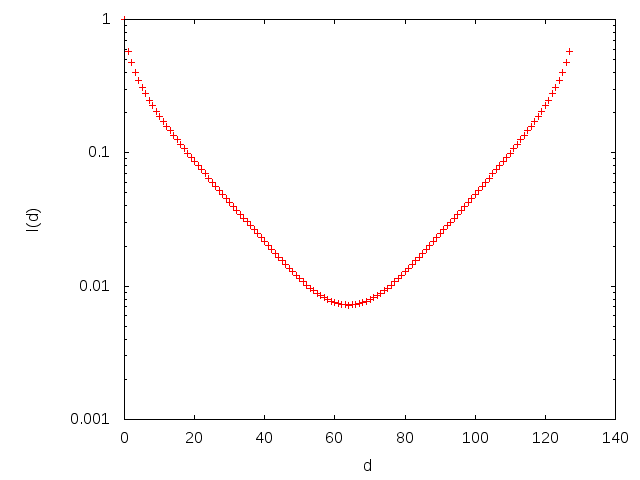
\includegraphics[width=0.8\textwidth] {images/Maths_Project_G5}
\caption{Eigenvalues for the correlator function with $\Phi_i(t) = \{\gamma_5\}$}
\end{figure}

\begin{figure}
\centering
	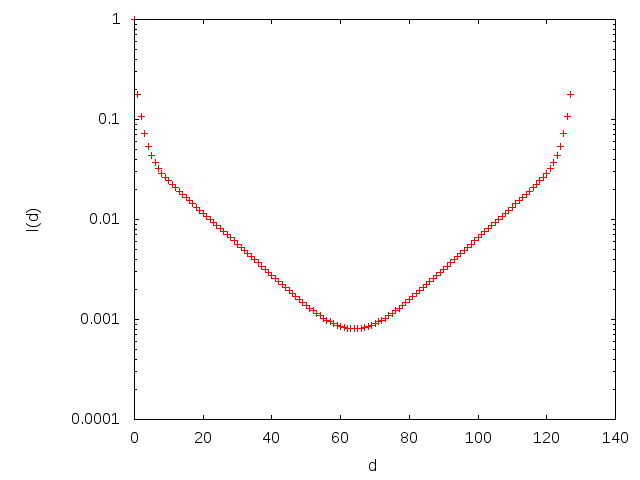
\includegraphics[width=0.8\textwidth] {images/Maths_Project_iG0G5}
\caption{Eigenvalues for the correlator function with $\Phi_i(t) = \{i\gamma_0\gamma_5\}$}
\end{figure}

\begin{figure}
\centering
	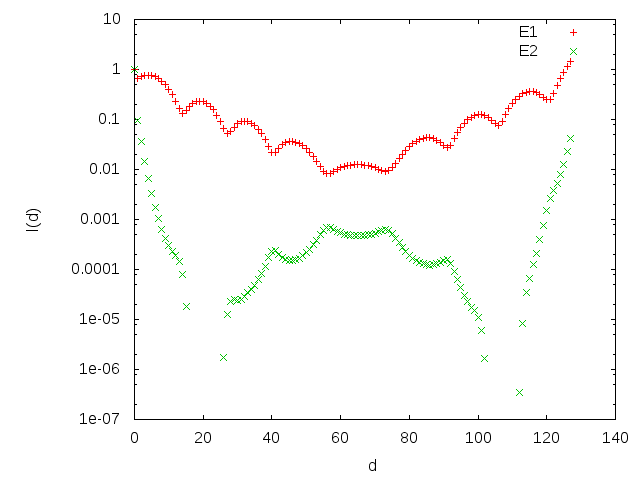
\includegraphics[width=0.8\textwidth] {images/Maths_Project_iG0G5_G5}
\caption{Eigenvalues for the correlator function with $\Phi_i(t) = \{i\gamma_0\gamma_5, \gamma_5\}$}\label{fig:iG0G5_G5}
\end{figure}


\bibliographystyle{plain}
\bibliography{Maths_Project}
\end{document}

##########################
##	Motivation	##
##########################
-Two point correlation functions

-Reduce loads on clusters, move it to desktop computers

-cheap GPU cards

-CUDA GPGPU

##################################
##	Parallel Programs	##
##################################
-Transform a for loop into a kernel
--limitations on allowed for loops

-Threads

-Different parallel paradigms
--SIMD
--MIMD
--Message Passing

##################################
##	NVIDIA Architecture	##
##################################
-Thread organization
--What is a thread?
--What is a block?
--What is a grid?

-Organization of memory on chips

-Access of memory (coalescing)

##########################################
##	The CUDA programming language	##
##########################################
-Memory allocations and movement

-grid and block dimensions

-launching a kernel

##################################################################################
##	Performance  Bottlenecks and optimizations (Problems and solutions)	##
##################################################################################
-Latency
--prefetching
--coalescing

-Bandwidth
--tiling

-Overhead
--kernel combining

-Register iteration
--loop unrolling

-Kernel divergence
--striding

-division and modulo
--bit shifting and bitwise and

-Dimension limitations
--divisions algorithm

##########################
##	The problem	##
##########################
-Grassman algebra
--useful identities

-Matrix formulation of Correlation function
--derivation

##########################
##	The solution	##
##########################
-Mapping of the functions to tensors

-Splitting up the tensors to fit on the card

-matrix valued rank 3 tensor multiplier

-tracing function for correlator
--performance considerations (need high C dim)

-Database loading
--parallel loading
--loading entirely into memory
--loading partially into memory

##########################
##	Results		##
##########################
-Does it at least work???